\let\lesson\undefined
\newcommand{\lesson}{\phantomlesson{Bài 10.}}
\setcounter{section}{2}
\section{Bài tập trắc nghiệm}
\begin{enumerate}[label=\bfseries Câu \arabic*:]
	\item \mkstar{1}\\
	{Đại lượng đặc trưng cho mức quán tính của một vật là
		\begin{mcq}(4)
			\item trọng lượng.
			\item khối lượng.
			\item vận tốc.
			\item lực.
		\end{mcq}
	
}
\hideall{
\textbf{Đáp án: B.}
}

\item \mkstar{2}\\
{Phát biểu nào sau đây là đúng?
	\begin{mcq}
		\item Nếu không chịu lực nào tác dụng thì vật phải đứng yên.
		\item Nếu không chịu lực nào tác dụng thì vật phải đứng yên.
		\item Khi vận tốc của vật thay đổi thì chắc chắn đã có lực tác dụng lên vật.
		\item Khi không chịu lực nào tác dụng lên vật thì vật đang chuyển động sẽ lập tức dừng lại.
	\end{mcq}

}
\hideall{
\textbf{Đáp án: C.}
}

\item\mkstar{2}\\
{Trong chuyển động thẳng chậm dần đều thì hợp lực tác dụng vào vật
	\begin{mcq}
		\item cùng chiều với chuyển động.
		\item cùng chiều với chuyển động và có độ lớn không đổi.
		\item ngược chiều với chuyển động và có độ lớn nhỏ dần.
		\item ngược chiều với chuyển động và có độ lớn không đổi.
	\end{mcq}

}
\hideall{
\textbf{Đáp án: D.}
}

\item\mkstar{2}\\
{Nếu một vật đang chuyển động có gia tốc mà lực tác dụng lên vật tăng lên thì vật sẽ thu được gia tốc 
	\begin{mcq}(2)
		\item nhỏ hơn.
		\item lớn hơn.
		\item bằng 0.
		\item không đổi.
	\end{mcq}

}
\hideall{
\textbf{Đáp án: B.}
}

\item \mkstar{2}\\
{Hợp lực của tất cả các lực tác dụng lên vật
	\begin{mcq}
		\item có hướng trùng với hướng chuyển động của vật.
		\item có hướng không trùng với hướng chuyển động của vật.
		\item có hướng trùng với hướng của gia tốc mà vật thu được.
		\item khi vật chuyển động thẳng đều có độ lớn thay đổi.
	\end{mcq}

}
\hideall{
\textbf{Đáp án: C.}
}

\item \mkstar{2}\\
{Một người tiếp viên hàng không đang đẩy một chiếc xe đẩy xuống lối đi của một chiếc máy bay đang bay. Khi xác định gia tốc của xe đẩy so với máy bay thì ta không cần chú ý đến dữ kiện nào sau đây?   
	\begin{mcq}(2)
		\item Lực ma sát của bánh xe với mặt sàn.  
		\item Lực mà người tiếp viên tác dụng lên xe đẩy.  
		\item Vận tốc của máy bay.  
		\item Khối lượng của xe đẩy và hàng hoá trên đó. 
	\end{mcq}
	
}
\hideall{
	\textbf{Đáp án: C.}
}

\item\mkstar{3}\\
{Một vật có khối lượng $\SI{2}{\kilogram}$ chuyển động thẳng nhanh dần đều từ trạng thái nghỉ. Vật đi được $\SI{100}{\centi\meter}$ trong $\SI{0.25}{\second}$. Gia tốc của vật và hợp lực tác dụng lên vật có giá trị lần lượt là
	\begin{mcq}(4)
		\item $\SI{32}{\meter/\second^2}$; $\SI{64}{\newton}$.
		\item $\SI{0.64}{\meter/\second^2}$; $\SI{1.2}{\newton}$.
		\item $\SI{6.4}{\meter/\second^2}$; $\SI{12.8}{\newton}$.
		\item $\SI{64}{\meter/\second^2}$; $\SI{128}{\newton}$.
	\end{mcq}

}
\hideall{
\textbf{Đáp án: A.}
}

\item\mkstar{3}\\
{Một quả bóng đang nằm yên trên  mặt đất thì bị một cầu thủ đá bằng một lực $\SI{13.5}{\newton}$ và bóng thu được gia tốc $\SI{6.5}{\meter/\second^2}$. Bỏ qua mọi ma sát. Khối lượng của bóng là
	\begin{mcq}(4)
		\item $\SI{2.08}{\kilogram}$.
		\item $\SI{0.5}{\kilogram}$.
		\item $\SI{0.8}{\kilogram}$.
		\item $\SI{5}{\kilogram}$.
	\end{mcq}

}
\hideall{
\textbf{Đáp án: A.}
}

\item \mkstar{3}\\
{Lần lượt tác dụng lực có độ lớn $F_1$ và $F_2$ lên một vật khối lượng $m$, vật thu được gia tốc có độ lớn lần lượt là $a_1$ và $a_2$. Biết $1,5F_1=F_2$. Bỏ qua mọi ma sát. Tỉ số $\dfrac{a_2}{a_1}$ là
	\begin{mcq}(4)
		\item $\dfrac{3}{2}$.
		\item $\dfrac{2}{3}$.
		\item $3$.
		\item $\dfrac{1}{3}$.
	\end{mcq}

}
\hideall{
\textbf{Đáp án: A.}
}

\item \mkstar{3}\\
{Một lực không đổi tác dụng vào một vật có khối lượng $\SI{2.5}{\kilogram}$ làm vận tốc của nó tăng dần từ $\SI{2}{\meter/\second}$ đến $\SI{6}{\meter/\second}$ trong $\SI{2}{\second}$. Lực tác dụng vào vật có độ lớn bằng 
	\begin{mcq}(4)
		\item $\SI{7.5}{\newton}$.
		\item $\SI{5}{\newton}$.
		\item $\SI{0.5}{\newton}$.
		\item $\SI{2.5}{\newton}$.
	\end{mcq}

}
\hideall{
\textbf{Đáp án: B.}
}

\item \mkstar{3}\\
{Một hợp lực $\SI{2}{\newton}$ tác dụng vào một vật có khối lượng $\SI{2}{\kilogram}$ lúc đầu đứng yên, trong khoảng thời gian $\SI{2}{\second}$. Đoạn đường mà vật đó đi được trong khoảng thời gian đó là
\begin{mcq}(4)
	\item $\SI{8}{\meter}$.
	\item $\SI{2}{\meter}$.
	\item $\SI{1}{\meter}$.
	\item $\SI{4}{\meter}$.
\end{mcq}
}
\hideall{
\textbf{Đáp án: B.}
}

\item \mkstar{3}\\
{Một ô tô khối lượng 1 tấn đang chuyển động với tốc độ $\SI{72}{\kilo\meter/\hour}$ thì hãm phanh chuyển động thẳng chậm dần đều và đi thêm được $\SI{500}{\meter}$ rồi dừng lại. Chọn chiều dương là chiều chuyển động. Lực hãm tác dụng lên xe là
	\begin{mcq}(4)
		\item $\SI{800}{\newton}$.
		\item $\SI{-800}{\newton}$.
		\item $\SI{400}{\newton}$.
		\item $\SI{-400}{\newton}$.
	\end{mcq}

}
\hideall{
\textbf{Đáp án: D.}
}

\end{enumerate}
\section{Bài tập tự luận}
\begin{enumerate}[label=\bfseries Bài \arabic*:]
	\item \mkstar{1}
	
	{
		Trong trò chơi thổi viên bi, mỗi bạn sử dụng một ống bơm khí từ vật liệu đơn giản như hình, thổi khí vào viên bi được đặt trên ray định hướng. Người chơi sẽ chiến thắng khi thổi viên bi đi xa hơn sau ba lần. Hãy sử dụng định luật II Newton giải thích làm thế nào để có thể chiến thắng trò chơi này.
		\begin{center}
			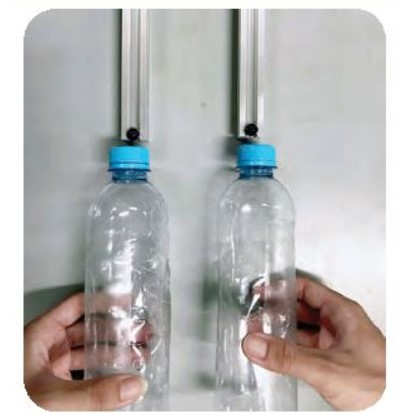
\includegraphics[scale=0.6]{../figs/VN10-2022-PH-TP017-5.jpg}
		\end{center}
	}
	
	\hideall{
		
		Áp dụng định luật II Newton, ta có lực càng lớn thì gia tốc càng lớn, vật sẽ càng đi được xa. Ta bóp ở cuối chai thì sẽ tạo ra lực lớn.
		
	}

	\item \mkstar{2}
	
	
	{Cho đồ thị biểu diễn mối liên hệ giữa các lực tác dụng lên một vật và gia tốc gây ra tương ứng. Khối lượng của vật là bao nhiêu?
		
		\begin{center}
			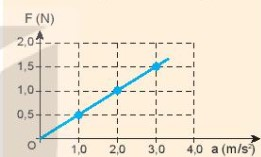
\includegraphics[scale=1]{../figs/VN10-2022-PH-TP017-2.jpg}
		\end{center}
	}
	
	\hideall
	{	
		
		Khối lượng của vật là
		
		$$m = \dfrac{F_1}{a_1} = \dfrac{F_2}{a_2} = \dfrac{F_3}{a_2} = \dfrac{\text{0,5}}{\text{1,0}} = \dfrac{\text{1,0}}{\text{2,0}} =\dfrac{\text{1,5}}{\text{3,0}} = \SI{0,5}{kg}.$$
		
	}

	\item \mkstar{2}
	
	{
		
		Một lực có độ lớn $\SI{6}{N}$ tác dụng lên vật có khối lượng $\SI{0,5}{kg}$ đang đứng yên. Bỏ qua ma sát và các lực cản. Gia tốc của vật bằng bao nhiêu?
		
	}
	
	\hideall{
		
		Gia tốc của vật là:
		
		$$a = \dfrac{F}{m} = \SI{12}{m/s}^2.$$
	}
	\item \mkstar{3}
	
	{
		Xét một ô tô có khối lượng $\SI{900}{kg}$ đang đi với vận tốc $\SI{20}{m/s}$ thì người lái xe nhìn thấy đèn giao thông chuyển màu đỏ ở phía trước. Để xe giảm tốc độ và dừng lại sau $\SI{10}{s}$ thì lực hãm khi phanh ô tô phải là bao nhiêu?
	}
	
	\hideall{
		
		Gia tốc của ô tô cần có để giảm tốc và dừng lại là:
		
		$$a = \dfrac{\Delta v}{\Delta t} = -\SI{2}{m/s}^2.$$
		
		Lực hãm phanh được xác đinh:
		
		$$F = ma = - \text{1,8} \cdot 10^3\ \text{N}.$$
		
		Như vậy, độ lớn lực hãm khi phanh là $\text{1,8}\cdot 10^3\ \text{N}$ để xe giảm tốc và dừng lại sau $\SI{10}{s}$ từ vận tốc $\SI{20}{m/s}$. Dấu "=" thể hiện lực ngược chiều chuyển động, gây ra gia tốc ngược hướng vận tốc.
	}
	
	\item \mkstar{3}
	
	{
		
		Mẫu xe điện có thời gian tăng tốc nhanh nhất được thử nghiệm đã tăng tốc từ $\SI{0}{km/h}$ đến $\SI{97}{km/h}$ trong 1,98 giây. Hãy tính gia tốc của xe và lực để tạo ra gia tốc đó. Coi xe chuyển động biến đổi đều và khối lượng của mẫu xe này là 2 tấn.
	}
	
	\hideall{
		
		Đổi $\SI{97}{km/h} = \SI{26,94}{m/s}.$
		
		Ta có:
		
		$$a = \dfrac{v - v_0}{t} = \SI{13,61}{m/s}^2.$$
		
		Mà: 
		
		$$F = ma = \SI{27220}{\newton}$$
		
	}
	\item \mkstar{3}
	
	{
		
		Thông số mẫu xe ô tô được cung cấp như bảng dưới đây. Tính lực tác dụng để mẫu xe trên chở đủ tải trọng và tăng tốc từ trạng thái nghỉ đến tốc độ tối ưu trong 2 giây.
		
		\begin{center}
			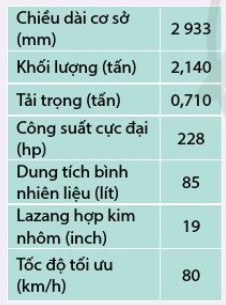
\includegraphics[scale=1]{../figs/VN10-2022-PH-TP016-1.jpg}
		\end{center}
		
	}
	
	\hideall{
		
		Để xe trên chở đủ tải trọng và tăng tốc từ trạng thái nghỉ đến tốc độ tối ưu trên 2 giây thì gia tốc của xe là:
		
		$$a = \dfrac{v - v_0}{t} = \SI{11,11}{m/s}^2.$$
		
		Lực tác dụng là
		
		$$F = ma= \SI{31666.6}{\newton}.$$
	}
	\item \mkstar{3}
	
	{
		
		Một người có khối lượng $\SI{60}{kg}$ đi trên xe đạp có khối lượng $\SI{20}{kg}$. Khi xuất phát, hợp lực tác dụng lên xe đạp là $\SI{200}{N}$. Giả sử hợp lực tác dụng lên xe đạp không đổi, hãy tính vận tốc của xe đạp sau $\SI{5}{s}$.
	}
	
	\hideall{
		
		Xe đạp đi với gia tốc là:
		
		$$a=\dfrac{F}{m}= \SI{2,5}{m/s}^2.$$
		
		Vận tốc của xe đạp sau $\SI{5,00}{s}$ là:
		
		$$v=v_0+at = \SI{12,5}{m/s}.$$
		
	}
	
	\item \mkstar{3}
	
	{
		
		Một ô tô có khối lượng 1 tấn đang chuyển động với $v = \SI{54}{km/h}$ thì tắt máy, hãm phanh, chuyển động chậm dần đều. Biết độ lớn lực hãm $\SI{3000}{N}$. Xác định quãng đường xe đi được cho đến khi dừng lại.
	}
	
	\hideall{
		
		Do đây là lực hãm nên sẽ mang giá trị âm.
		
		Gia tốc của vật:
		
		$$a = \dfrac{-F}{m} = -\SI{3}{m/s}^2.$$
		
		Khi xe dừng ta có $v=0$ ta có:
		
		$$s = \dfrac{v^2 - v_0^2}{2a} = \SI{37,5}{m}.$$
	}
	
	\item \mkstar{3}
	
	{
		
		Lực không đổi tác dụng vào vật $m_1$ gây gia tốc $\SI{4}{m/s}^2$; tác dụng vào vật $m_2$ gây ra gia tốc $\SI{5}{m/s}^2.$ Tính gia tốc của vật có khối lượng $m_1 + m_2$ chịu tác dụng của lực trên.
	}
	
	\hideall{
		
		Ta có:
		
		$$a = \dfrac{F}{m_1 + m_2} = \dfrac{F}{\dfrac{F}{a_1}+ \dfrac{F}{a_2}} = \dfrac{1}{\dfrac{1}{a_1}+ \dfrac{1}{a_2}} = \SI{0,22}{m/s}^2.$$
		
	}
\item \mkstar{3}


{Một xe tải khối lượng 1 tấn, sau khi khởi hành được $10\ \text s$ đạt vận tốc $18\ \text{km/h}$. Biết lực cản mà mặt đường tác dụng lên xe là $500\ \text N$. Tính lực phát động của động cơ.
}

\hideall
{	Gia tốc của xe:
	\[a = \dfrac{v-v_0}{\Delta t} = \dfrac{1}{2}\ \text{m/s}^2\]
	
	Mà $F-F_\text c = ma \Rightarrow F = F_\text c + ma = 500 + 500 = 1000\ \text N$
}

\end{enumerate}